\documentclass{beamer}
\usepackage[french]{babel}
\usepackage[utf8]{inputenc} 
\usepackage[T1]{fontenc}
\usepackage{tikz}
\usepackage{times}
\usepackage{listings}

\usetikzlibrary{arrows,positioning}

\usetheme{Madrid}
\setbeamertemplate{blocks}[rounded][shadow=true]

\lstset{language=Python, basicstyle=\footnotesize\ttfamily}

\title[OSGi, iPOJO]{OSGi Concepts \& iPOJO Components}
\author{Thomas Calmant}
\date{}

\AtBeginSection[]{
  \begin{frame}
  \vfill
  \centering
  \begin{beamercolorbox}[sep=8pt,center,shadow=true,rounded=true]{title}
    \usebeamerfont{title}\insertsectionhead\par%
  \end{beamercolorbox}
  \vfill
  \end{frame}
}

\begin{document}
\titlegraphic{
	
\includegraphics[width=.3\textwidth]{../imgs/ipojo_logo}
}
\frame{\titlepage}
\frame{\frametitle{Agenda}\tableofcontents}

%----------------------------------------
% OSGi
%----------------------------------------
\section{OSGi}
\subsection{Service-Oriented Architecture}

\begin{frame}{Service-Oriented Architecture}
\begin{block}{Principles}
\begin{itemize}
\item Bindings based on provided contracts
\item Loose Coupling: no knowledge of implementation details
\end{itemize}
\end{block}

\begin{block}{Service Registry}
\begin{itemize}
\item Keeps track of contract providers and consumers
\item Late binding: at runtime, on demande
\end{itemize}
\end{block}
\end{frame}

\begin{frame}{Service Registry}
\begin{center}

\tikzset{
    %Define standard arrow tip
    >=stealth',
    %Define style for boxes
    punkt/.style={
           rectangle,
           rounded corners,
           draw=black, very thick,
           text width=6.5em,
           minimum height=2em,
           text centered},
    % Define arrow style
    pil/.style={
           ->,
           thick,
           shorten <=2pt,
           shorten >=2pt,}
}

\begin{tikzpicture}
\node[punkt] (R) at (4, 4) {Service Registry};
\node[punkt, blue] (C) at (0, 0) {Service Consumer};
\node[punkt, red] (P) at (8, 0) {Service Provider};

\draw[pil, bend right=45]
    (P.north) to node[auto, swap] {\texttt{Provides}}(R.east);
\draw[pil, <->, bend left=45]
    (C.north) to node[auto] {\texttt{Looks up}}(R.west);
\draw[pil, -] (C.east) to node[auto] {\texttt{Binds \& Uses}}(P.west);
\draw[very thick, blue] (2, .4) arc (90:270:2ex);
\filldraw[very thick, red] (6, 0) circle (2ex);
\end{tikzpicture}
\end{center}
\end{frame}


\subsection{OSGi: SOA in Java}

\begin{frame}{OSGi: Concepts}
\begin{block}{SOA Principles Equivalents}
\begin{center}
\begin{tabular}{rp{.5\textwidth}}
Contract & Java Interface\\
\hline
Service & Object implementing an Interface\\
\hline
Registry & Framework service registry\\
\end{tabular}
\end{center}
\end{block}

\begin{block}{Concepts}
\begin{center}
\begin{tabular}{rp{.6\textwidth}}
Framework & Services \& bundles registry\\
\hline
Bundle & JAR file providing Java interfaces, classes and resources\\
\hline
Bundle Context & Link between bundle classes and the framework\\
\hline
Service & Object implementing an interface, associated to properties\\
\end{tabular}
\end{center}
\end{block}
\end{frame}

\begin{frame}{OSGi Ecosystem}
\begin{block}{Specifications}
\begin{itemize}
\item Definition of services behaviours, interfaces and properties
\item Multiple overlapping specification levels:
\begin{itemize}
\item Core: main concepts, framework behavior and core services
\item Compendium: additional core services (log service, remote services, \ldots)
\item Enterprise: additional services (security management, \ldots)
\item Redidential: services for IoT and Home Automation
\end{itemize}
\end{itemize}
\end{block}

\begin{block}{Major Implementations}
\begin{center}
\begin{tabular}{rl}
Equinox & Eclipse Foundation\\
Felix & Apache Software Foundation\\
Concierge & ETH Zurich\\
Knopflerfish & Makewave\\
\end{tabular}
\end{center}
\end{block}
\end{frame}

\begin{frame}{OSGi Bundle}
\centering
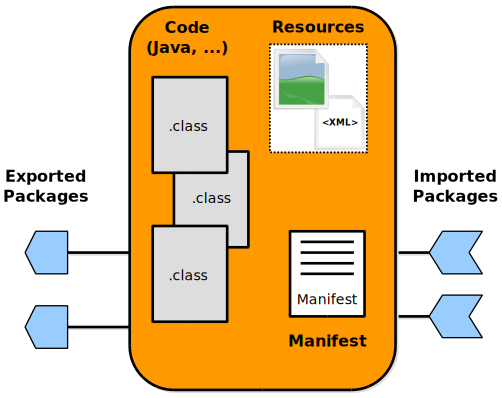
\includegraphics[height=.8\textheight]{../imgs/bundle}
\end{frame}

\begin{frame}{OSGi Bundle Manifest}
\begin{block}{Common Manifest Entries}
\begin{center}
\begin{tabular}{rp{.6\textwidth}}
Bundle-SymbolicName & Identifier of the bundle\\
Bundle-Version & Normalized version number \par (\textit{major.minor.micro-qualifier})\\
Import-Package & List of required packages, with a version\\
Export-Package & List of provided packages, with a version\\
\end{tabular}
\end{center}
\end{block}

\begin{block}{Optional Entries}
\begin{center}
\begin{tabular}{rp{.6\textwidth}}
Bundle-Name & Human-readable name\\
Bundle-Description & Long description\\
Bundle-Vendor & Name of the bundle provider\\
\end{tabular}
\end{center}
\end{block}
\end{frame}

\begin{frame}{OSGi Bundle Life Cycle}
\centering

\tikzset{
    %Define standard arrow tip
    >=stealth',
    %Define style for boxes
    punkt/.style={
           rectangle,
           rounded corners,
           draw=black, very thick,
           fill=yellow!30,
           text width=6.5em,
           minimum height=2em,
           text centered},
    % Define arrow style
    pil/.style={
           ->,
           thick,
           shorten <=2pt,
           shorten >=2pt,}
}

\begin{tikzpicture}[node distance=2.5em, auto]
\node[circle, draw, very thick, fill=yellow!30] (init) {};
\node[punkt, below=of init] (installed) {INSTALLED};
\node[punkt, below=of installed] (resolved) {RESOLVED};
\node[punkt, below=of resolved] (uninstalled) {UNINSTALLED};
\node[punkt, right=of installed] (starting) {STARTING};
\node[punkt, right=of resolved] (active) {ACTIVE};
\node[punkt, right=of uninstalled] (stopping) {STOPPING};
\node[circle, draw, very thick, fill=black, below=of uninstalled] (final) {};

\draw[pil] (init.south) to node[auto, swap] {Install} (installed.north);
\draw[pil, <->] (installed.south) to node[auto, swap] {Resolve} (resolved.north);
\draw[pil] (resolved.east) to node[auto] {Start} (starting.west);
\draw[pil] (starting.south) to node[auto] {} (active.north);
\draw[pil] (active.south) to node[auto] {Stop} (stopping.north);
\draw[pil] (stopping.west) to node[auto] {} (resolved.east);
\draw[pil] (resolved.south) to node[auto, swap] {Uninstall} (uninstalled.north);
\draw[pil, bend right=35] (installed.west) to node[auto, swap] {Uninstall} (uninstalled.west);
\draw[pil] (uninstalled.south) to node[auto] {} (final.north);
\end{tikzpicture}
\end{frame}


\subsection{Code Snippets}

\begin{frame}[fragile]{Snippets: Bundle Activator}
\begin{small}
\begin{block}{mypackage/MyActivator.java}
\begin{minted}{java}
public class MyActivator implements BundleActivator {
	public void start(BundleContext ctxt) {
		System.out.println("Bundle Started");
	}
	public void stop(BundleContext ctxt) {
		System.out.println("Bundle Stopped");
	}
}
\end{minted}
\vspace{-.8em}
\end{block}
\begin{block}{META-INF/MANIFEST.MF}
\begin{minted}{yaml}
Manifest-Version: 1.0
Bundle-ManifestVersion: 2
Bundle-SymbolicName: net.coderxpress.snippets.activator
Bundle-Version: 1.0.0
Bundle-Activator: mypackage.MyActivator
Bundle-RequiredExecutionEnvironment: JavaSE-1.6
\end{minted}
\vspace{-.8em}
\end{block}
\end{small}
\end{frame}


\begin{frame}[fragile]{Snippets: Un/register a service}
\begin{small}
\begin{block}{Register a service}
\begin{minted}{java}
// Instantiate the service object
MyInterface service = new MyImplementation();

// Set up properties
Hashtable properties = new Hashtable();
properties.put("answer", 42);

// Register the service
ServiceRegistration<MyInterface> svcReg = ctxt.registerService(
	MyInterface.class, service, properties);
\end{minted}
\vspace{-.8em}
\end{block}

\begin{block}{Unregister a service}
\begin{minted}{java}
// Unregister the service
svcReg.unregister();
\end{minted}
\vspace{-.8em}
\end{block}
\end{small}
\end{frame}

\begin{frame}[fragile]{Snippets: Consume a service}
\begin{small}
\begin{block}{Find a Service}
\begin{minted}{java}
// Find the first service matching an interface and/or properties
svcRef = ctxt.getServiceReference(
	MyInterface.class.getName(), "(answer=42)");
\end{minted}
\vspace{-.8em}
\end{block}

\begin{block}{Consume a Service}
\begin{minted}{java}
// Get the service
MyInterface service = ctxt.getService(svcRef);

// Use it
service.hello("world");

// Release it
ctxt.ungetService(svcRef);
service = null;
\end{minted}
\vspace{-.8em}
\end{block}
\end{small}
\end{frame}


%----------------------------------------
% iPOJO
%----------------------------------------
\section{iPOJO}
\subsection{Service-Oriented Component Model}

\begin{frame}{iPOJO: Service-Oriented Component Model in Java}
\begin{block}{iPOJO Concepts}
\begin{tabular}{lp{.7\textwidth}}
Component & Instance of a \textit{Factory} class\\
\hline
Factory & (Annotated) Java class, modified by iPOJO after compilation\\
\hline
Handler & Manages a component according to information in its Factory\\
\end{tabular}
\end{block}

\begin{block}{Features}
\begin{itemize}
\item Components are bound by services
\item All the binding and life-cycle management is done by handlers
\item The Factory class only has to provide the business code
\end{itemize}
\end{block}
\end{frame}

\begin{frame}{Component Overview}
\centering
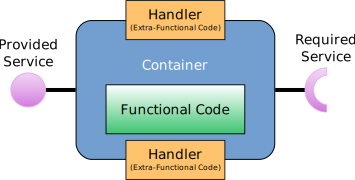
\includegraphics[width=\textwidth]{../imgs/cbse_component}
\end{frame}

\begin{frame}{Component Life Cycle}
\centering

\tikzset{
    %Define standard arrow tip
    >=stealth',
    %Define style for boxes
    punkt/.style={
           rectangle,
           rounded corners,
           draw=black, very thick,
           fill=yellow!30,
           text width=7em,
           minimum height=2em,
           text centered},
    % Define arrow style
    pil/.style={
           ->,
           thick,
           shorten <=2pt,
           shorten >=2pt,}
}

\begin{tikzpicture}[node distance=2.5em, auto]
\node[circle, draw, very thick, fill=yellow!30] (init) {};
\node[punkt, below=of init] (instantiated) {INSTANTIATED};
\node[punkt, right=10em of init] (validating) {VALIDATING};
\node[punkt, below=of validating] (valid) {VALID};
\node[punkt, below=of valid] (invalidating) {INVALIDATING};
\node[punkt, below=of instantiated] (deleted) {DELETED};
\node[circle, draw, very thick, fill=black, below=of deleted] (final) {};

\draw[pil] (init.south) to node[auto, swap] {Instantiate} (instantiated.north);
\draw[pil] (instantiated.east) to node[auto] {Validate} (validating.west);
\draw[pil] (validating.south) to node[auto] {} (valid.north);
\draw[pil] (valid.south) to node[auto] {Invalidate} (invalidating.north);
\draw[pil] (invalidating.west) to node[auto] {} (instantiated.east);
\draw[pil] (instantiated.south) to node[auto, swap] {Remove} (deleted.north);
\draw[pil] (deleted.south) to node[auto] {} (final.north);
\end{tikzpicture}
\end{frame}

\subsection{Code Snippets}

\begin{frame}[fragile]{Snippet: Sample Provider}
\begin{block}{Hello world sample}
\begin{minted}{java}
@Component(name="my-provider"}
@Provides(specification=MyInterface.class)
@Instantiate(name="my-provider-instance")
public class MyImplementation implements MyInterface {

	@Requires(optional=true)
	private LogService logger;
	
	public void hello(String name) {
		System.out.println("Hello, " + name + "!");
		logger.log(LogService.LOG_DEBUG,
			"Said hello to " + name);
	}
}
\end{minted}
\end{block}
\end{frame}

\begin{frame}[fragile]{Snippet: Sample Consumer}
\begin{block}{Hello world sample}
\begin{minted}{java}
@Component(name="my-consumer"}
@Instantiate(name="my-consumer-instance")
public class MyConsumer {
	@Requires
	private MyInterface service;
	
	@Property(name = "my.name", value = "World")
	private String name;
	
	@Validate
	public void validated() {
		System.out.println("Consumer validated!");
		service.hello(name);
	}
	
	@Invalidate
	public void validated() {
		System.out.println("Consumer invalidated!");
		service.hello("the end");
	}
}
\end{minted}
\end{block}
\end{frame}

\begin{frame}[fragile]{Snippet: Result}
\begin{block}{Hello world sample}
\begin{minted}{bash}
$ install file:ipojo.jar
Bundle ID 5
$ start 5

$ install file:consumer.jar
Bundle ID 6
$ start 6

$ install file:provider.jar
Bundle ID 7
$ start 7
Consumer validated!
Hello, World!

$ stop 7
Consumer invalidated!
Hello, the end!
\end{minted}
\end{block}
\end{frame}


%----------------------------------------
% Questions
%----------------------------------------
\begin{frame}
  \vfill
  \centering
  \begin{beamercolorbox}[sep=8pt,center,shadow=true,rounded=true]{title}
    \usebeamerfont{title}Questions ?\par%
  \end{beamercolorbox}
  \vspace{3ex}
  
\includegraphics[width=.5\textwidth]{../imgs/questions_fry}
  \vfill
\end{frame}
\end{document}
